\documentclass[tikz,border=5mm]{standalone}

% \usepackage{fontawesome5} % For the gear icon
\usepackage{fontawesome} % For the gear icon
\usetikzlibrary{positioning, shapes, arrows.meta, calc}

\begin{document}

\begin{tikzpicture}[font=\sffamily]

    % -------------------------------------------------------------- %
    % Define styles for nodes and arrows
    % -------------------------------------------------------------- %
    \tikzstyle{process} = [rectangle, draw, minimum width=2.5cm, minimum height=1cm]
    \tikzstyle{arrow} = [thick,->, line width=1mm, >=Latex, scale=2]
    \tikzstyle{gear} = [font=\Large] % For larger gear icons

    % -------------------------------------------------------------- %
    % draw the coordinate and grid
    % -------------------------------------------------------------- %
    % \draw[->] (0,0) -- (0,1);
    % \draw[->] (0,0) -- (1,0);
    % \draw[color=gray, style=dotted] (0,0) grid[xstep=1, ystep=1] (15,-5);

    % -------------------------------------------------------------- %
    % draw the document files configure.ac and Makefile.am
    % -------------------------------------------------------------- %
    \node (config-ac-symbol) at (0,0) { \Huge  \faFileTextO };
    \node (configure-ac-text) [below of=config-ac-symbol] {configure.ac};

    \node (makefile-am-symbol) [below of=configure-ac-text, yshift=-0.5cm] { \Huge \faFileTextO };
    \node (makefile-am-text) [below of=makefile-am-symbol] {Makefile.am};

    % -------------------------------------------------------------- %
    % draw running autoreconf
    % -------------------------------------------------------------- %
    \node (autoreconf-text) [right of=configure-ac-text, xshift=2cm] {autoreconf};
    \node (gear-one) [gear, above of=autoreconf-text, node distance=0.5cm] {\faCog};
    \node (gear-two) [gear] at ($(gear-one.north east) + (-0.05, -0.05)$ ){\faCog};

    % -------------------------------------------------------------- %
    % draw the document file configure and Makefile.in
    % -------------------------------------------------------------- %
    \node (configure-text) [right of=autoreconf-text, node distance=3cm] {configure};
    \node (config-symbol) [ above of=configure-text] { \Huge  \faFileTextO };
    
    \node (makein) [right of=makefile-am-text, node distance=6cm] {Makefile.in};
    \node (makefile-in-symbol) [above of=makein] { \Huge \faFileTextO  };

    % -------------------------------------------------------------- %
    % draw running configuration 
    % -------------------------------------------------------------- %
    \node (run-configure) [right of=configure-text, node distance=3cm] {./configure};
    
    % % Gears next to configure
    \node (gear-three) [gear, above of=run-configure, node distance=0.5cm] {\faCog};
    \node (gear-four) [gear] at ($(gear-three.north east) + (-0.05, -0.05)$) {\faCog};

    % -------------------------------------------------------------- %
    % draw final generated Makefile
    % -------------------------------------------------------------- %
    \node (finalmake) [right of=run-configure, node distance=3cm, yshift=-1cm] {Makefile};
    \node (makefile-symbol) [above of=finalmake, node distance=1cm] { \Huge \faFileTextO };

    % -------------------------------------------------------------- %
    % draw arrow from configure.ac to configure
    % -------------------------------------------------------------- %
    \draw[arrow] 
    let \p1 = (configure-ac-text.south east),
        \p2 = (configure-text.south west) in
    (\x1, \y1-8) -- (\x2, \y1-8);

    \draw[arrow]
    let \p1 = (configure-text.south east),
        \p2 = (finalmake.south west) in
    (\x1, \y1-8) -- (\x2, \y1-8);

\end{tikzpicture}

\end{document}
